\section{Pattern Client-Server}
\begin{figure}[H] 
    \centering 
    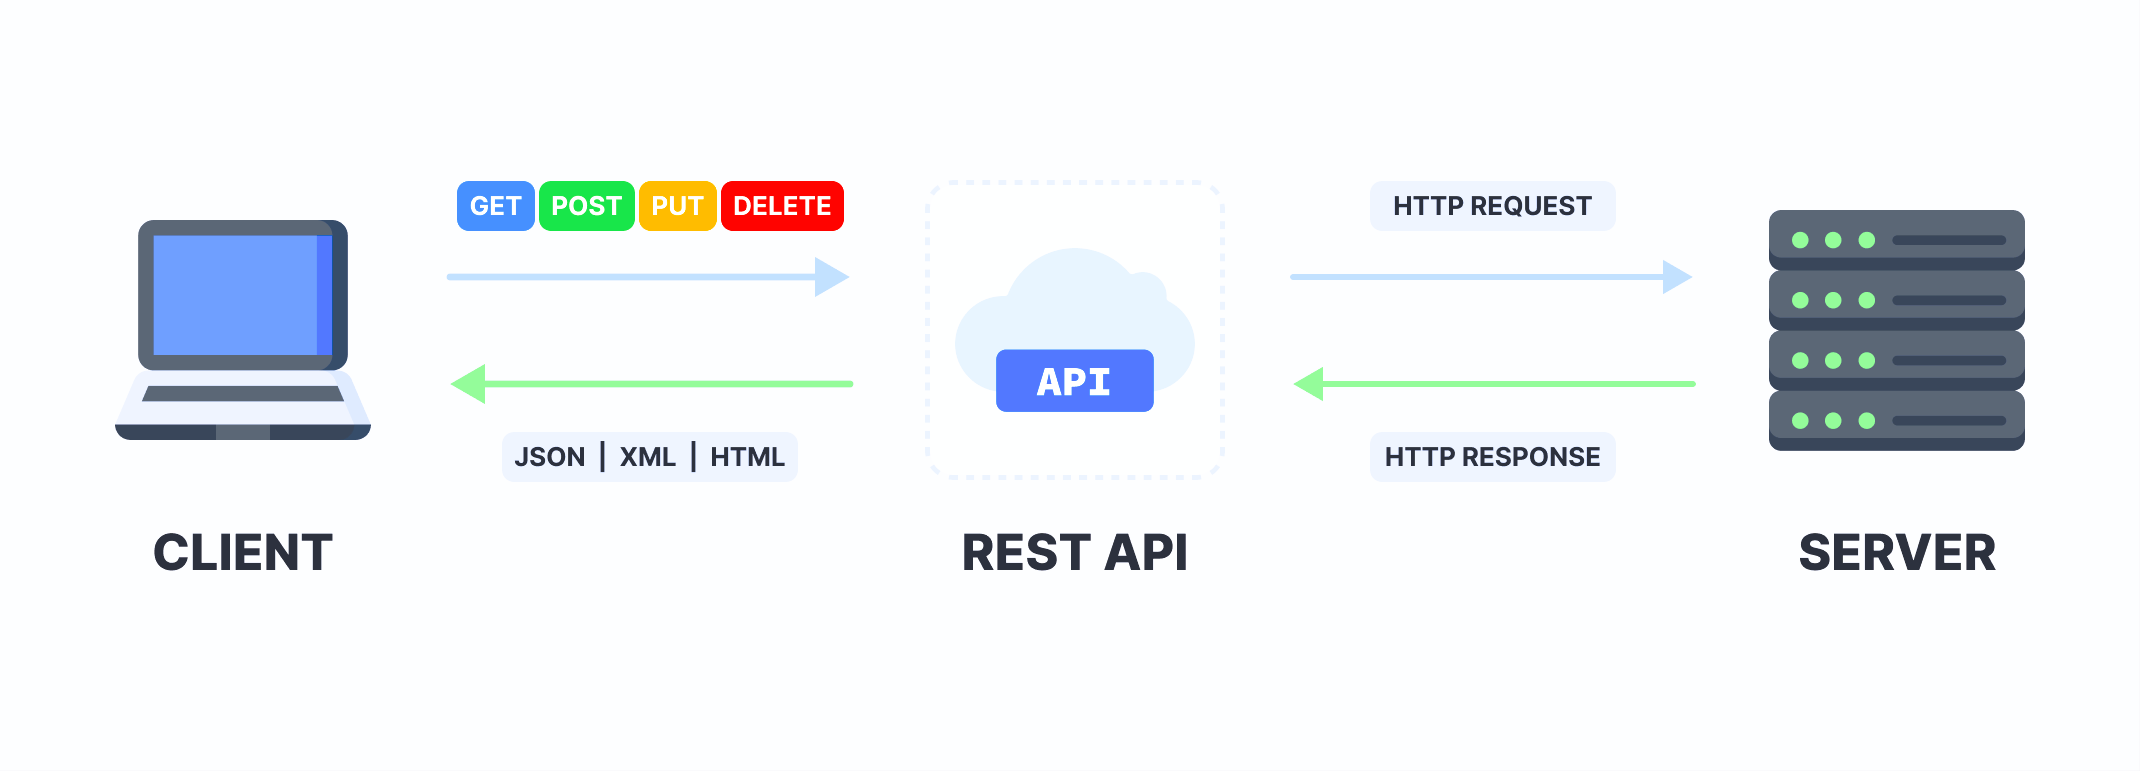
\includegraphics[width=0.90\columnwidth]{client-server} 
    \caption{Client-Server in una REST API}
\end{figure}
È un pattern architetturale composto da due componenti: client e server. Il client rappresenta il richiedente del servizio, mentre il server fornisce i contenuti e i servizi ai client, restando in attesa delle loro richieste.\\
Il pattern client-server si adatta perfettamente ad una API REST e le sue componenti sono identificate in questo modo.
\subsection*{Client}
In questo contesto il client è rappresentato da applicazioni o servizi che comunicano con l'API REST, inviando le richieste HTTP al server per ottenere quanto richiesto. Il client invia richieste utilizzando verbi standard HTTP per accedere alle risorse e alle funzionalità che l'API offre.
\subsection*{Server} 
Il server invece è colui che gestisce le richieste HTTP ricevute e genera le risposte in formato JSON. Esso quindi elabora le richieste ed interagisce col database per recuperare le informazioni.\\